\documentclass[12pt, a4paper]{article}
\usepackage{graphicx}
\usepackage{mathtools}
\usepackage{amsmath}
\usepackage{geometry}
\linespread{1.1}
\usepackage{caption}
\usepackage[italian]{babel}

\geometry{
 total={170mm,257mm},
 left=20mm,
 top=15mm,
 bottom=28mm
 }
\title{\textbf{\scalebox{1.4}{\text{{\Huge Pendolo}}}}}
\date{}
\author{\begin{small}Mussini Simone, Ruscillo Fabio, Musi Francesco\end{small}}
\begin{document}
\maketitle



\section{Richiami teorici}
Il pendolo semplice è un sistema costituito da un filo inestensibile di lunghezza $L$ di massa trascurabile a cui è appesa una massa $m$, che all'occorrenza può essere spostata dalla posizione verticale di equilibrio e dare origine ad un moto oscillatorio. 

Trascurando l'attrito con l'aria, sulla massa agisce soltanto la forza peso. 
L'equazione del moto si ottiene egualiando la compnente normale della forza rispetto al filo, alla formula generica per la forza centripeta di un moto circolare con raggio = $L$.
Risulta essere un moto armonico soltanto per le piccole oscillazioni, cioè quando si può approssimare $sin(\theta) = \theta$, dove $\theta$ è l'angolo che il filo forma con la verticale. 

\begin{equation}
        F_t = -mg sin(\theta)\hat{t} = mL\ddot{\theta}   \quad \xrightarrow{} \quad   \frac{d^2\theta}{dt^2} = -\omega^2\theta 
\end{equation}

Dove $\omega = \sqrt{\frac{g}{L}}$ è la pulsazione, che dipende non dalla massa $m$, ma soltanto dalla lunghezza del filo e accelerazione di gravità. 

Il periodo di una oscillazione risulta: $T = \frac{2\pi}{\omega} = 2\pi\sqrt{\frac{L}{g}}$.





\section{Obbiettivi}
Gli obbiettivi di questo esperimento sono: 
verificare l'indipendenza del periodo $T$, tenendo $L$ costante, dall'ampiezza delle oscillazioni e dalla massa;
verificare la relazione quadratica tra $L$ e $T$; 
verificare il valore $g$ tramite na linearizzazione (quadratica) della legge del periodo.


\section{Strumenti}
    \begin{itemize}
        \item Piedistallo 
        \item filo inestensibile
        \item Masse calibrate
        \item Cronometro 
        \item Goniometro 
    \end{itemize}

    
\section{Procedimento di misura}
Il setup dell'esperimento è costituito da un piedistallo a cui è collegato un filo inestensibie regolabile in lunghezza tramite una vite. Nell'estremità superiore è presente un goniometro, solidale con il piedistallo, che permette di sapere l'angolo delle oscillazioni. All'estremità inferiore del filo è collegata una spilla che permette di variare la massa appesa. \\
Disponiamo di 5 masse che pesano: 66.3g, 37.2g, 22.2g, 16.8g, 12.5g.

Sui dati presi con il cronometro, consideriamo l'errore umano nella misura dei tempi, ossia un decimo di secondo, maggiore dell'errore strumentale. 
Nella misura degli angoli con il goniometro, tenimao l'errore trumentale. 

Abbiamo notato che la lunghezza del filo, aumenta all'aumentare della massa. Tuttavia la discrepanza tra allungamento massimo e minimo è minore della somma dei rispettivi errori ($\pm0.2cm$ su ogni misura), quindi possiamo approssimarlo a filo inestensibile.

Le masse le assumiamo note essendo l'ordine di grandezza dell'errore relativo trascurabile.

Per aumentare la precisione delle misure, è opportuno misurare 10 periodi alla volta.
Infatti, visto che un periodo è nell'ordine di 1 secondo, misurando un oscillazione alla volta, con l'errore umano si avrebbe un errore relativo dell'ordine del 10\%, troppo alto.
Invece essendo $10T$ nell'ordine di 10 secondi, l'errore relativo scende all'1\% circa.

È importante anche avere $L > 1m$, in modo che le oscillazioni non siano troppo brevi, sempre per tenere basso l'errore relativo.


\section{Analisi preliminare}
Fissati L, g e $\Phi_{max}$, va verificato che le 30 misure di $10T$ prese siano una popolazione gaussiana, per poter eseguire le regressioni lineari e di potenza che serviranno successivamente. Riportiamo i dati in tabella. 


\begin{table}[!htb]
    \begin{minipage}[t]{.3\linewidth}
    \centering
        \begin{tabular}{|c|c|}
            \hline
            $10T$ $(s)$&$N$\\
            \hline
            $20.67$ & $1$\\
            $20.72$ & $1$\\
            $20.76$ & $1$\\
            $20.87$ & $1$\\
            $20.93$ & $1$\\
            $21.00$ & $2$\\
            $21.07$ & $1$\\
            \hline
        \end{tabular}
    \end{minipage}
    \begin{minipage}[t]{.3\linewidth}
    \centering
        \begin{tabular}{|c|c|}
            \hline
            $10T$ $(s)$&$N$\\
            \hline
            $21.09$ & $2$\\
            $21.13$ & $2$\\
            $21.14$ & $1$\\
            $21.16$ & $2$\\
            $21.20$ & $1$\\
            $21.25$ & $2$\\
            $21.26$ & $3$\\
            \hline
        \end{tabular}
    \end{minipage}
    \begin{minipage}[t]{.3\linewidth}
    \centering
        \begin{tabular}{|c|c|}
            \hline
            $10T$ $(s)$&$N$\\
            \hline
            $21.27$ & $1$\\
            $21.33$ & $2$\\
            $21.42$ & $1$\\
            $21.43$ & $1$\\
            $21.52$ & $2$\\
            $21.59$ & $1$\\
            $21.78$ & $1$\\
            \hline
        \end{tabular}
    \end{minipage} 
\end{table}

Successivamente si  verificato se fossero una poolazione gaussiana, ...... FINISCI !!!






\section{Indipendenza di T da $\Phi_{max}$}

\section{Relazione tra T ed L}

\section{Misura di g}














\newpage
\section{RELAZIONE MOLLA PER COPIARE TABELLE}
Questo step consiste nel misurare l'allungamento delle due molle soggette a differenti forze, generate dai contrappesi. I dati sono riportati di seguito in Tabella \ref{tab: Misure Statiche Non Precompresse} e Tabella \ref{tab: Misure Statiche Precompresse}:
\\

\begin{table}[!htb]
    \begin{minipage}[t]{.5\linewidth}
    \centering
        \begin{tabular}{|c|c|}
        \hline
        $M$ $(kg)$&$L\pm \Delta L$ $(m)$\\
        \hline
        $0.050$ & $0.326$$\pm$$0.002$\\
        $0.100$ & $0.346$$\pm$$0.002$\\
        $0.150$ & $0.366$$\pm$$0.002$\\
        $0.200$ & $0.387$$\pm$$0.002$\\
        $0.250$ & $0.407$$\pm$$0.002$\\
        $0.300$ & $0.427$$\pm$$0.002$\\
        $0.350$ & $0.448$$\pm$$0.002$\\
        $0.400$ & $0.468$$\pm$$0.002$\\
        $0.450$ & $0.489$$\pm$$0.002$\\
        $0.500$ & $0.509$$\pm$$0.002$\\
        \hline
    \end{tabular}
    \captionsetup{width=7cm}
    \caption{Molla Non Precompressa. Sono riportati la massa e la posizione finale misurata in seguito alla deformazione.}

    \label{tab: Misure Statiche Non Precompresse}
    \end{minipage}
    \begin{minipage}[t]{.5\linewidth}
    \centering
        \begin{tabular}{|c|c|}
            \hline
            $M$ $(kg)$&$L\pm \Delta L$ $(m)$\\
            \hline
            $0.050$ & $0.203$$\pm$$0.003$\\
            $0.100$ & $0.203$$\pm$$0.003$\\
            $0.150$ & $0.203$$\pm$$0.003$\\
            $0.200$ & $0.208$$\pm$$0.003$\\
            $0.250$ & $0.224$$\pm$$0.003$\\
            $0.300$ & $0.242$$\pm$$0.003$\\
            $0.350$ & $0.259$$\pm$$0.003$\\
            $0.400$ & $0.276$$\pm$$0.003$\\
            $0.450$ & $0.295$$\pm$$0.003$\\
            $0.500$ & $0.313$$\pm$$0.003$\\
            \hline
        \end{tabular}
        \captionsetup{width=7cm}
        \caption{Molla Precompressa. Al di sotto di una massa pari a $0.150$ $kg$ non si è ossservata alcuna deformazione della molla.}
        
        \label{tab: Misure Statiche Precompresse}
    \end{minipage} 
\end{table}






\subsection{Relazione tra T ed L}
Dato che la legge di Hook $Mg=K_s\cdot(L-L_0)$ ci suggerisce che l'allungameto sia in relazione lineare con la forza applicata, abbiamo attuato una regressione lineare. 
Per la molla non precompressa la legge di cui trovare i coefficienti è: 
\begin{equation*}
    L=M\cdot\displaystyle\frac{g}{K_s}+L_0
    \xrightarrow{} Y = A + BX
\end{equation*} 
dove\\ 
\begin{equation*}
 A= L_0 \mbox{ , } B=\displaystyle\frac{g}{K_s} \mbox{ , } y = L \mbox{ e } X = m
\end{equation*}



\begin{figure}[h]
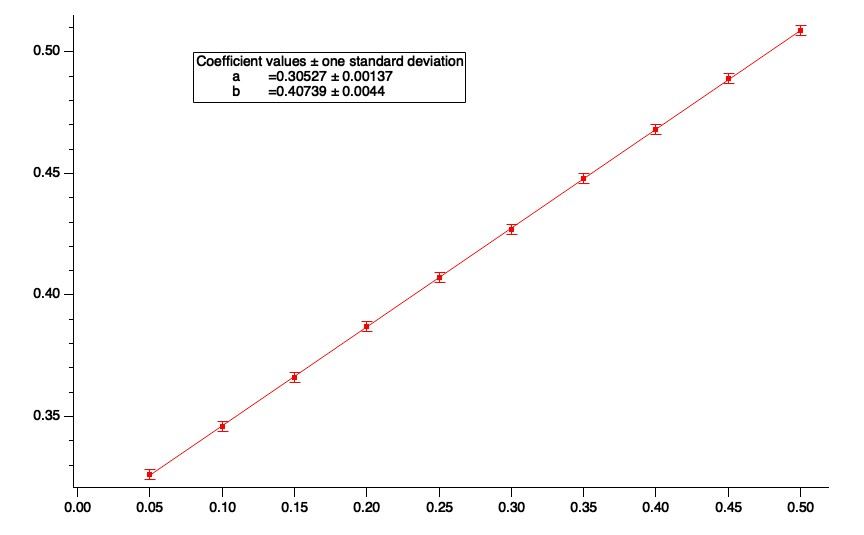
\includegraphics[width=170mm]{IMMAGINI/Graph Molla Arm Stat.jpg}
\centering
\caption{\textit{{\footnotesize{Grafico $L(M)$}: sul'asse asse \textit{y} sono riportati i valori della posizione finale misurata $L$ coi rispettivi errori, sull'asse \textit{x} la massa corrispettiva}}}
\label{Grafico parabolico}
\end{figure}


\bigskip
\bigskip


Calcolando $K_s$ e il rispettivo errore $\Delta K_s$ come\\

\begin{equation*}
\centering
    K_s= \frac{g}{B} \text{\phantom{Testo invi}} \text{,} \text{\phantom{Testo sibil}} \Delta K_s = \left | \frac{g}{B}  \right | \cdot \Delta B 
\end{equation*}
\bigskip

Si ottiene $K_s = (24.1 \pm 0.2)$ $N m^{-1}$






\subsection{Molla Precompressa - metodo statico}
Nel caso di una molla precompressa, la legge che lega l'allungamento alla forza applicata differisce dalla legge di Hooke per un termine costante $\frac{F_0}{K_p}$ , dovuto alla forza $F_0$ di precompressione della molla.  
\\La legge su cui abbiamo eseguito la regressione lineare risulata quindi: 
\begin{equation}
    L = m \frac{g}{k_p} + (L_0 - \frac{F_0}{K_p}) 
\end{equation}
dove 
\begin{equation}
    A = L_0 + \frac{F_0}{K_p} \  \ \ \   e   \ \ \ \ B = \frac{g}{K_p}
\end{equation}
\\Calcolando $K_p$ e il rispettivo errore $\Delta K_p$ come : 
\begin{equation}
    K_p = \frac{g}{B} e \Delta K_p = \left | \frac{g}{B}  \right | \cdot \Delta B 
\end{equation}






\section{Misura della costante elastica con metodo dinamico }
Questo step consiste nel misurare il tempo impiegato dalla molla, alla quale è fissato un pesetto da $500kg$, a compiere dieci oscillazioni complete. Al fine di ricavare la costante $k_d$ dalla relazione: 
\begin{equation}
    T = 2\pi \cdot \sqrt{\frac{k_d}{m}}
\end{equation} 

Per avere una miglior stima del periodo, abbiamo misurato 30  volte il tempo relativo alle 10 oscillazioni, inserendoli con le relative frequenze di misura, nella Tabella \ref{tab: Misure Dinamiche} a fine paragrafo.  

Abbiamo controllato che il campione fosse compatibile con una distribuzione gaussiana.
Calcolando il valore medio $\overline{x}$ e la deviazione standar $\sigma_x$ tramite le formule: 
\begin{equation}
    \overline{x} = \frac{\sum_{i=1}^{N}x_i}{N} \mbox{\hspace{0.5cm} , \hspace{0.5cm}}
    \sigma_x = \sqrt{\frac{\sum_{i=1}^{N}(x_i-\overline{x})^2}{(N-1)}}
\end{equation}

\smallskip
Nel nostro caso $\overline{x} = 9,2773$ e $\sigma_x = 0,0921 $. 
Ora possiamo dividere le misure delle dieci oscilazioni in classi con il relativo numero valori osservatie  riportarle  nella seguente tabella  


\begin{table}[hbt!]
    \centering
    {\renewcommand\arraystretch{1.0} 
    \begin{tabular}{|c|c|}
    \hline
        \textbf{Dieci Periodi} & \textbf{Frequenza}\\
        $10T(s)$ & $f(n)$\\
    \hline
    $ 9.07 $ & $ 1 $ \\ 
    $ 9.12 $ & $ 1 $ \\
    $ 9.13 $ & $ 1 $ \\
    $ 9.15 $ & $ 1 $ \\ 
    $ 9.21 $ & $ 1 $ \\
    $ 9.22 $ & $ 1 $ \\
    $ 9.23 $ & $ 3 $ \\
    $ 9.25 $ & $ 1 $ \\
    $ 9.26 $ & $ 3 $ \\
    $ 9.27 $ & $ 1 $ \\
    $ 9.28 $ & $ 2 $ \\
    $ 9.29 $ & $ 1 $ \\
    $ 9.30 $ & $ 3 $ \\ 
    $ 9.31 $ & $ 2 $ \\
    $ 9.32 $ & $ 2 $ \\
    $ 9.35 $ & $ 2 $ \\
    $ 9.37 $ & $ 1 $ \\
    $ 9.38 $ & $ 1 $ \\
    $ 9.47 $ & $ 1 $ \\
    $ 9,50 $ & $ 1 $ \\ 
    \hline
    \end{tabular}}
    \caption{Misurazioni dinamiche.}
    \label{tab: Misure Dinamiche}
\end{table}


\begin{table}[hbt!]
    \centering
    {\renewcommand\arraystretch{1.0} 
    \begin{tabular}{|c|c|}
    \hline
        \ & \textbf{}
        $10T(s)$ & $f(n)$\\
    \hline 
    \hline
    \end{tabular}}
    \caption{Misurazioni dinamiche.}
    \label{tab: Classi}
\end{table}



\newpage
\section{Determinazione di una massa incognita}
Questa misura consiste nell'appendere la massa e misurarne l'allungamento ($\Delta L$). Per calcolare il valore di $m_i$ bisogna usare la relazione lineare del paragrafo 5.1, in quanto anche questa è stata una misura statica. I coefficienti sono già stati trovati e riportati qui sotto. 
Il processo è stato svolto con la molla non precompressa, e sulla massa incognita compariva la lettera "A".\\

\begin{equation}
    L = A + Bm  \mbox{\hspace{0.5cm} quindi \hspace{0.5cm}}  m_i = \frac{L - A}{B}
\end{equation}\\

Con i valori: $A = (0.3052 \pm 0.0011)m$, $B = (0.407 \pm 0.004)\frac{m}{kg}$, $L = (0.517 \pm 0.002)m$, calcolando l'errore sommando le derivate parziali oltiplicate per gli errori relativi, si ottiene: 

\begin{equation} 
    m_i = (0.520 \pm 0.013)kg 
\end{equation}




\end{document}

